\subsection{2(a) $\lx{^R}{\pmb \omega}^B = \lx{^R}{\pmb \omega}^A + \lx{^A}{\pmb \omega}^B = \Omega A_3 +\dot \theta_1 X_1 + \dot \theta_2 X_2 + \dot \theta_3 X_3$
}

\itbf{Problem}: In Figure~\ref{2_a}, P represents a point fixed in a reference frame R, and $B^*$ designates the mass center of a rigid body $B$ that moves on a circular orbit $C$ fixed in $R$ and centered at $P$. $A_1, A_2$ and $A_3$ are mutually perpendicular directed line segments, $A_1$ being the extension of line $PB^*$, $A_2$ pointing in the direction of motion of $B^*$ on $C$, and $A_3$ thus being normal to the plane of the orbit $B^*$.

\begin{figure}[H]
    \centering
    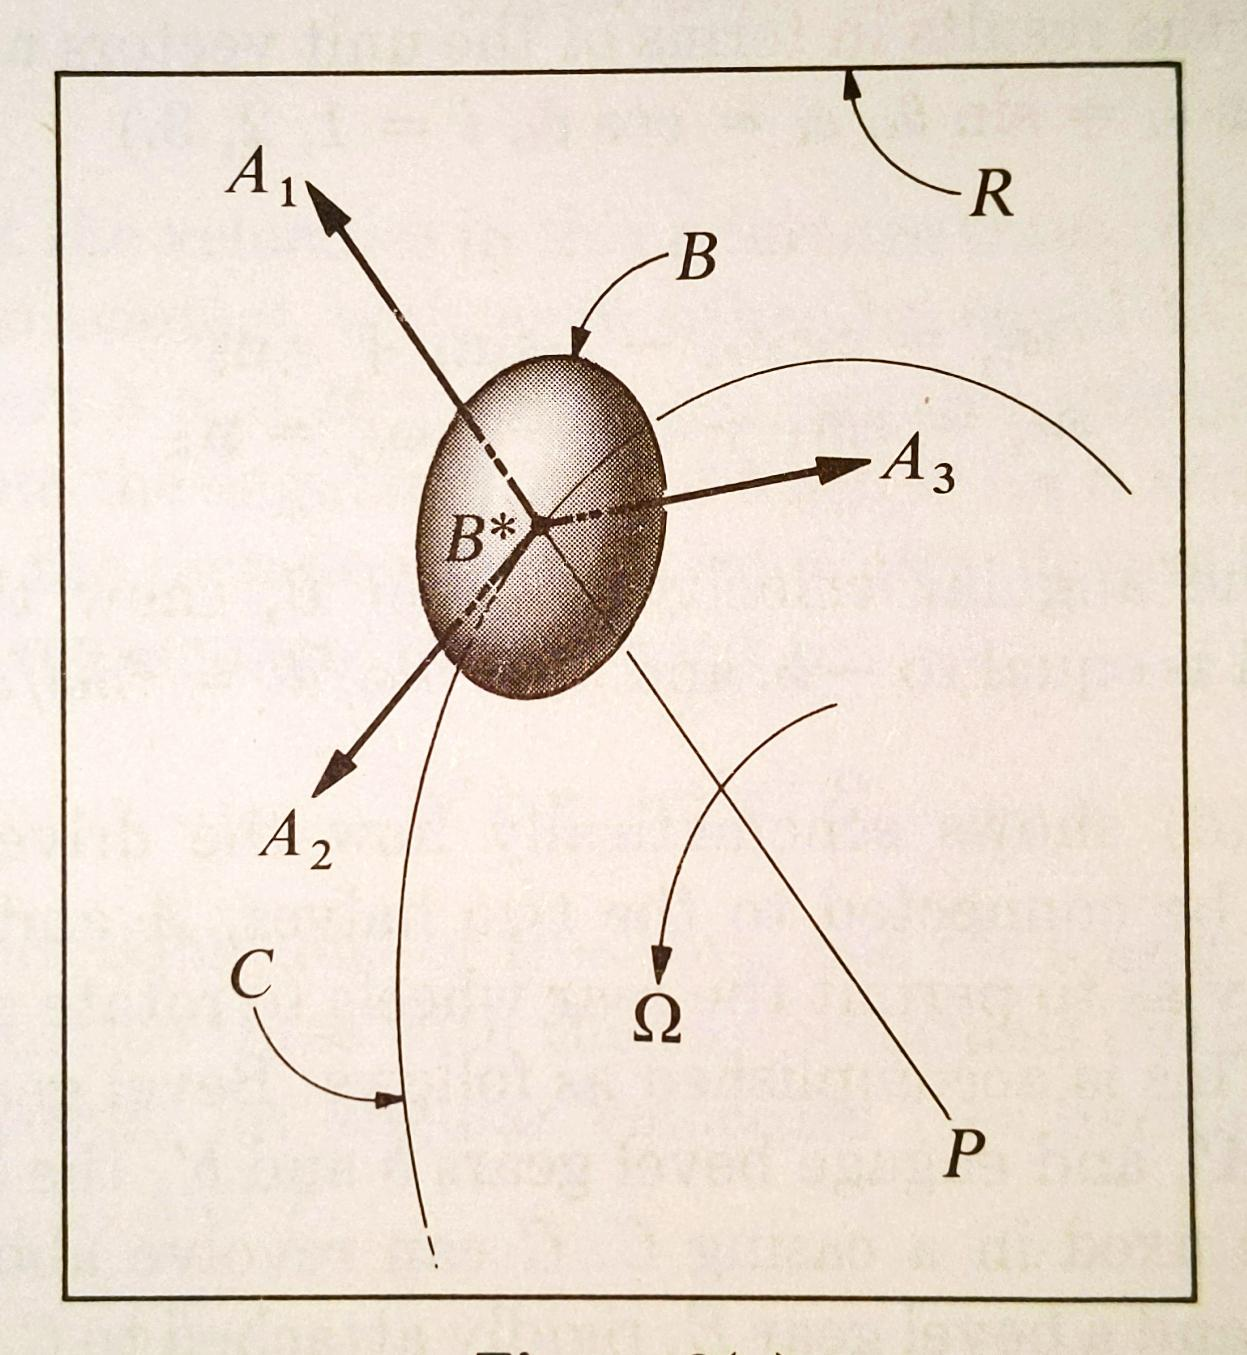
\includegraphics[scale = 0.15]{./figs/ProbSet_2/2_a.jpg}
    \caption{}
    \label{2_a}
\end{figure}

If $X_1, X_2$ and $X_3$ are mutually perpendicular directed line segments passing through $B^*$ and fixed in the body $B$, the "attitude" of $B$ relative to $A_1, A_2, A_3$ can be specified in terms of three angles $\theta_1, \theta_2$ and $\theta_3$, generated as follows: \itbf{Align $X_i$ with $A_i$, for $i=1, 2, 3$, and perform successive right-handed rotations of $B$, of amount $\theta_1$ about $X_1$, $\theta_2$ about $X_2$, and $\theta_3$ about $X_3$.}

The angular velocity $\pmb \omega$ of $B$ in $R$ can be expressed as $\pmb \omega = \omega_1 \pmb n_1 + \omega_2 \pmb n_2 + \omega_3 \pmb n_3$, where $\pmb n_i$ is a unit vector parallel to $X_i$, and $\omega_i$ is a function of $\theta_1, \theta_2, \theta_3, \dot \theta_1, \dot \theta_2, \dot \theta_3$, and the anglular speed $\Omega$ of the line $PB^*$ in R. Consequently, $\dot \theta_i$ can be expressed as a function $f_i$ of $\theta_1, \theta_2, \theta_3, \omega_1, \omega_2, \omega_3$, $i = 1,2,3$ and $\Omega$.

Determine the functions $f_1, f_2$ and $f_3$, using the abbrivations $s_i = \sin \theta_i, c_i = \cos \theta_i$ for $i = 1,2,3$, to state the results.\\

\itbf{Sol.}:\\

\itbf{Note}: The above explanation of $X_1, X_2$ and $X_3$ is the loose definition of Euler angles used to define the orientation of a rigid body.\\

\itbf{Rotation Matrices}:

The given description of obtaining the attitude of the body can be put mathematically uising rotation matrices as follows:

\begin{multicols}{2}
 \begin{enumerate}
    \item Right-handed rotation about $X_1$ by $\theta_1$:
    \begin{align*}
        \bm{X_1\\ X_2\\ X_3^{'}} &=
        \underbrace{\bm{1 & 0 & 0\\
                        0 & c_1 & s_1\\
                        0 & -s_1 & c_1}}_{R_1}
        \bm{A_1\\ A_2\\ A_3}
    \end{align*}
    \item Right-handed rotation about $X_2$ by $\theta_2$:
    \begin{align*}
        \bm{X_1^{'}\\ X_2\\ X_3} &=
        \underbrace{\bm{c_2 & 0 & -s_2\\
                        0 & 1 & 0\\
                        s_2 & 0 & c_2}}_{R_2}
        \bm{X_1\\ X_2\\ X_3^{'}}
    \end{align*}
    \item Right-handed rotation about $X_3$ by $\theta_3$:
    \begin{align*}
        \bm{X_1^{''}\\ X_2^{'}\\ X_3} &=
        \underbrace{\bm{c_3 & s_3 & 0\\
                        -s_3 & c_3 & 0\\
                        0 & 0 & 1}}_{R_3}
        \bm{X_1^{'}\\ X_2\\ X_3}
    \end{align*}
\end{enumerate}

\itbf{Interpretation}: $\pmb n_i$ are the unit vectors parallel to $X_i$ after the above transformation sequence.\\
Thus,
\begin{align*}
    \bm{\pmb n_1 \\ \pmb n_2 \\ \pmb n_3} &= \bm{X_1^{''}\\ X_2^{'}\\ X_3}
\end{align*}
\end{multicols}

We have, the (instantaneous) angular velocity of the body in $A$ frame:
\begin{align*}
    \lx{^A}{\pmb \omega}^B &= \dot \theta_1 X_1 + \dot \theta_2 X_2 + \dot \theta_3 X_3
\end{align*}

The angular velocity of $A$ in $R$:
$$ \lx{^R}{\pmb \omega}^A = \Omega A_3$$

The angular velocity of the body in reference frame:
\begin{align*}
    lx{^R}{\pmb \omega}^B &= \lx{^R}{\pmb \omega}^A + \lx{^A}{\pmb \omega}^B\\
        &= \Omega A_3 +\dot \theta_1 X_1 + \dot \theta_2 X_2 + \dot \theta_3 X_3
\end{align*}

Requried form:
\begin{align*}
    \lx{^R}{\pmb \omega}^B &= \omega_1 \pmb n_1 + \omega_2 \pmb n_2 + \omega_3 \pmb n_3
\end{align*}

Thus we need to write $A_3, X_1, X_2$ and $X_3$ in terms of $\pmb n_1, \pmb n_2, \pmb n_3$.

\begin{multicols}{2}
From the third transformation:
\begin{align*}
    \bm{X_1^{'}\\ X_2\\ X_3} &=
                    \bm{c_3 & -s_3 & 0\\
                        s_3 & c_3 & 0\\
                        0 & 0 & 1}
    \bm{\pmb n_1 \\ \pmb n_2 \\ \pmb n_3}\\
    \implies X_2 &= s_3 \pmb n_1 + c_3 \pmb n_2 \qquad X_3 = \pmb n_3\\
         X_1^{'} &= c_3 \pmb n_1 - s_3 \pmb n_2
\end{align*}
From the second transformation:
\begin{align*}
    \bm{X_1\\ X_2\\ X_3^{'}} &=
        \bm{c_2 & 0 & s_2\\
            0 & 1 & 0\\
            -s_2 & 0 & c_2}
    \bm{X_1^{'}\\ X_2\\ X_3}\\
    \implies X_1 &= c_2 X_1^{'} + s_2 X_3\\
    \implies X_1 &= c_2(c_3 \pmb n_1 - s_3 \pmb n_2) + s_2 \pmb n_3
\end{align*}
\end{multicols}

\begin{align*}
    \bm{X_1\\ X_2\\ X_3} &= \underbrace{\bm{c_2 c_3 & -c_2 s_3 & s_2\\
                                s_3     & c_3      & 0\\
                                0       & 0        & 1}}_T
                            \bm{\pmb n_1 \\ \pmb n_2 \\ \pmb n_3}
\end{align*}

From the first transformation:
\begin{align*}
    \bm{A_1\\ A_2\\ A_3} &=
                    \bm{1 & 0 & 0\\
                        0 & c_1 & -s_1\\
                        0 & s_1 & c_1}
    \bm{X_1\\ X_2\\ X_3^{'}}
    \quad and \quad X_3^{'} = -s_2 X_1^{'} + c_2 X_3 = -s_2 (c_3 \pmb n_1 - s_3 \pmb n_2) + c_2 \pmb n_3\\
    \\
    \implies A_3 &= s_1 X_2 + c_1 X_3^{'} = s_1(s_3 \pmb n_1 + c_3 \pmb n_2 ) + c_1 (-s_2 (c_3 \pmb n_1 - s_3 \pmb n_2) + c_2 \pmb n_3)\\
    &= \underbrace{\bm{s_1 s_3 - c_1s_2c_3 & s_1c_3 + c_1 s_2 s_3 & c_1 c_2}}_{P^T}
        \bm{\pmb n_1 \\ \pmb n_2 \\ \pmb n_3}
\end{align*}

Substituting, and writing in matrix form:
\begin{align*}
    \omega_1 \pmb n_1 + \omega_2 \pmb n_2 + \omega_3 \pmb n_3 &= \Omega A_3 +\dot \theta_1 X_1 + \dot \theta_2 X_2 + \dot \theta_3 X_3\\
    %===
    \bm{\omega_1 & \omega_2 & \omega_3}  \bm{\pmb n_1 \\ \pmb n_2 \\ \pmb n_3}
    &= \Omega P^T  \bm{\pmb n_1 \\ \pmb n_2 \\ \pmb n_3}
        + \bm{\dot \theta_1 & \dot \theta_2 & \dot \theta_3} T \bm{\pmb n_1 \\ \pmb n_2 \\ \pmb n_3}\\
    %===
    \implies \bm{\omega_1 \\ \omega_2 \\ \omega_3} &= \Omega P + T^T  \bm{\dot \theta_1 \\ \dot \theta_2 \\ \dot \theta_3}\\
    %===
    \implies \bm{\dot \theta_1 \\ \dot \theta_2 \\ \dot \theta_3} &= [T^T]^{-1} \left(\bm{\omega_1 \\ \omega_2 \\ \omega_3} - \Omega P \right)
\end{align*}
Symbolically solving (using sympy), we get:
\begin{align*}
    \bm{\dot \theta_1 \\ \dot \theta_2 \\ \dot \theta_3}&=
    \left[\begin{matrix}\frac{\Omega \sin{\left(\theta_{2} \right)} \cos{\left(\theta_{1} \right)} + \omega_{1} \cos{\left(\theta_{3} \right)} - \omega_{2} \sin{\left(\theta_{3} \right)}}{\cos{\left(\theta_{2} \right)}}\\- \Omega \sin{\left(\theta_{1} \right)} + \omega_{1} \sin{\left(\theta_{3} \right)} + \omega_{2} \cos{\left(\theta_{3} \right)}\\- \frac{\Omega \cos{\left(\theta_{1} \right)}}{\cos{\left(\theta_{2} \right)}} - \omega_{1} \cos{\left(\theta_{3} \right)} \tan{\left(\theta_{2} \right)} + \omega_{2} \sin{\left(\theta_{3} \right)} \tan{\left(\theta_{2} \right)} + \omega_{3}\end{matrix}\right]
\end{align*}

Thus,
\begin{align*}
    \bm{\dot \theta_1 \\ \dot \theta_2 \\ \dot \theta_3}&=
    \bm{(\omega_1 c_3 - \omega_2 s_3 + \Omega s_2 c_1)/c_2 \\
        \omega_1 s_3 + \omega_2 c_3 - \Omega s_1 \\
        [(\omega_2 s_3 - \omega_1 c_3)s_2 + \omega_3 c_2 - \Omega c_1]/c_2}
\end{align*}

Sympy Code:
\lstinputlisting[language=python, caption ={}]{./ProblemSets/ProbSet_2/2a.py}
